\subsection{Fine-Tuning with Behavioral Cloning}
\label{section:BC_finetuning}
Foundation models are designed to have a broad behavior profile and be generally capable across a wide variety of tasks.
To incorporate new knowledge or allow them to specialize on a narrower task distribution, it is common practice to fine-tune these models to smaller, more specific datasets.\cite{brown2020language}
The VPT foundation model trained on the broad \texttt{web\_clean} dataset had nontrivial zero-shot performance; it was able to craft a crafting table yet unable to go past this in the technology tree.
As a case study into BC fine-tuning, we attempt to improve the VPT foundation model's ability to collect and craft these ``early game'' items by fine-tuning to two narrower datasets targeted at Minecraft behavior within the first few minutes of players starting in a fresh world.
In the first dataset, \texttt{contractor\_house}, contractors have 10 minutes to build a basic house from scratch using primarily wood, sand, and dirt.
Collecting contractor data can be difficult and expensive, so we also construct a dataset \texttt{earlygame\_keyword} by searching for videos online with descriptions that match keywords such as “new world”, “let's play episode 1”, etc.; this is a subset of \texttt{web\_clean} and is labeled with the IDM. See Appendix~\ref{appendix:contractor_house_data} and~\ref{appendix:early_game_data} for full descriptions of both datasets.

\begin{figure}[h]
\begin{center}
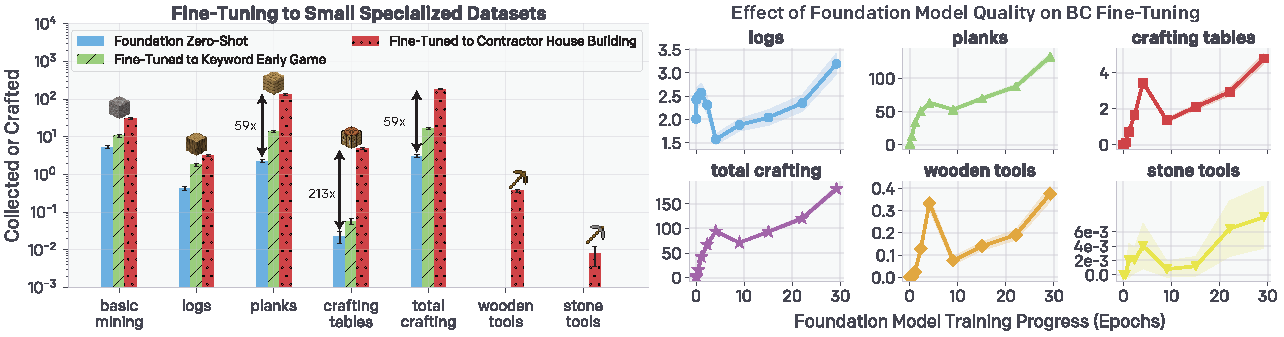
\includegraphics[width=\linewidth]{assets/Fine-Tuning_Main_Plot2.pdf}
\end{center}
\vspace{-8px}
\caption{\textbf{(Left)} Collection and crafting rates for three policies: the zero-shot VPT foundation model, and the VPT foundation model BC fine-tuned to the \texttt{earlygame\_keyword} or \texttt{contractor\_house} datasets. BC fine-tuning to either dataset improves performance, including (for the \texttt{contractor\_house} dataset) yielding wooden and stone tools.
Proficient Minecraft players take a median of 1.2 minutes (1390 actions) to construct wooden tools and 2.3 minutes (2790 actions) to construct stone tools. \textbf{(Right)} Collection and crafting rates for VPT foundation model snapshots throughout training \emph{after} they are BC fine-tuned to the \texttt{contractor\_house} dataset. In general, crafting-related behaviors increase throughout foundation model training. Fig.~\ref{fig:foundation} defines the other task terms (logs, planks, crafting tables, and total crafting).
}
\label{fig:main_finetuning}
\end{figure}

Fine-tuning to \texttt{earlygame\_keyword} results in a large boost compared to the zero-shot foundation model: 2.5x more crafting tables, 6.1x more planks, 4.3x more logs, and 5.5x more crafting overall (Fig.~\ref{fig:main_finetuning}).
However, when fine-tuning to this dataset we did not see any new behaviors emerge, only a refinement of existing skills. We saw an even bigger improvement when fine-tuning to the \texttt{contractor\_house} dataset: 213x more crafting tables, 59x more wooden planks, 7x more logs, and 59x more crafting over all. In addition, we saw the emergence of crafting wooden tools, which requires placing a crafting table on the ground, opening it to reveal a new crafting interface, and then using it to craft wooden tools. This entire sequence takes a proficient human player a median of 1.2 minutes (1390 consecutive actions) to accomplish. The model goes further and collects cobblestone, which requires a wooden pickaxe to mine, and crafts stone tools, requiring it to again use a crafting table; this takes a proficient human player a median of 2.3 minutes (2790 consecutive actions). We also saw this model more frequently raiding villages that randomly spawn in the game, hunting animals for food, in addition to many behaviors we saw performed by the foundation model.\footnote{Sample Videos: \href{https://www.youtube.com/playlist?list=PLNAOIb\_agjf2yDSs4AqcoyPv4z\_eWUiKm}{https://www.youtube.com/playlist?list=PLNAOIb\_agjf2yDSs4AqcoyPv4z\_eWUiKm}}

Despite the foundation model's zero-shot rollout performance plateauing 1/3 into training (Fig.~\ref{fig:foundation}, right), fine-tuning performance \textit{does} continue to increase throughout foundation model training (Fig.~\ref{fig:main_finetuning}, right).
Additionally, there is a stark difference in performance when training from scratch vs.\ fine-tuning from the VPT foundation model (Fig.~\ref{fig:main_finetuning} right, comparing the left and rightmost points).